\chapter{Test}   % ACHTUNG: fuer Dokumentclass FZGdasa hier \chapter verwenden (weils der Kong so will...), sonst immer \section
\label{sec:sektionsueberschrift}
%
Kapitelreferenz \chapref{sec:sektionsueberschrift} und eine Sectionsreferenz \secref{sec:paragraph} und noch ein Bild referenzieren: \figref{fig:beispiel} oder so \sfigref{fig:beispiel}
%
% ======================================================================================================
\section{Sektionsüberschrift}
\label{sec:nochmalsektion}
%
Literatur \cite{DIN3990} \cite{testweb}
%
%===================
\subsection{Subsektion}
\label{sec:subsektion}
%
\begin{figure}
	\centering
	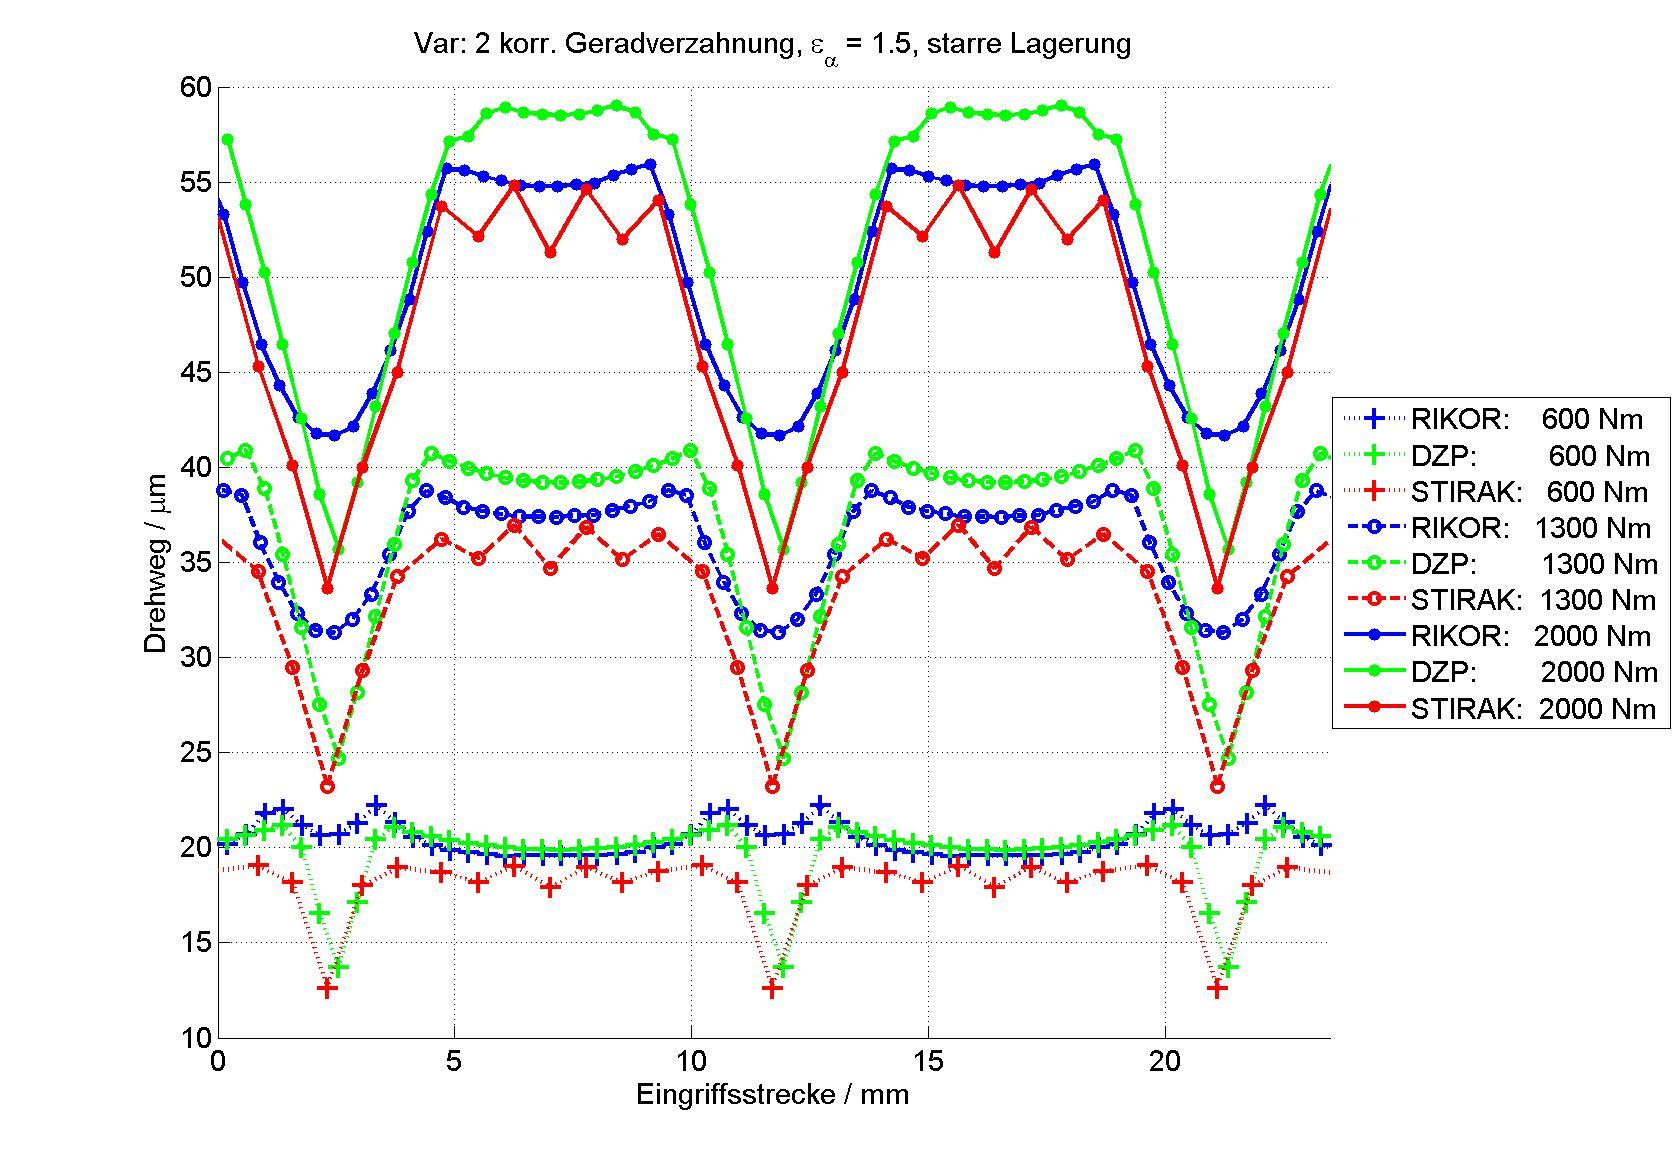
\includegraphics[width=0.5\textwidth]{_ltx/Beispiel.jpg}
	\caption{Dies ist ein wunderschönes Bild, das auch aus einer Quelle und so weiter stammen kann \cite{Niemann01}. Deshalb sind Bildunterschriften so einfach möglich.}
	\label{fig:beispiel}
\end{figure}
%
%----------------------
\subsubsection{Subsubsektion}
\label{sec:subsubsektion}
%
\textbf{fett} \textit{italic} \textsl{sl} \textsc{Kapitälchen}
%
%---------
\paragraph{Paragraph}
\label{sec:paragraph}
%
%
\newpage
\section{Formeln}
\label{sec:Formeln}
%
Das Beschreiben und Referenzieren von Formeln erfolgt nach DIN~1338.
%
\subsection{Beispiel nach DIN 1338}
%
In der Ausgleichsflächenformulierung wird der Polarwinkel über die Reihendarstellung
\begin{equation}
	\varphi_s = \sum_{j=0}^{m} \sum_{i=0}^{n} c_{ij} B_{i,n} B_{j,m}
	\label{eq:Polarwinkel}
\end{equation}
mit den Basispolynomen~$B_{i,n}$ und $B_{j,m}$ approximiert. Für die Wahl der Basispolynome eignen sich die Bernsteinpolynome
\begin{equation}
	B_{i,n}(t) = \binom{n}{i} t^i (1 - t)^{n - i}\text{,}
	\label{eq:Bernsteinpolynome}
\end{equation}
da sie die Eigenschaft der ‚Zerlegung der Eins‘ aufweisen. Die Basiskoeffizienten~$c_{ij}$ in \eqref{eq:Polarwinkel} können unter anderem mit der ‚Methode der kleinsten Fehlerquadrate‘ ermittelt werden:
\begin{equation}
	\sum_{s=1}^{q} (\varphi_s - \varphi)^2 = 0\text{.}
	\label{eq:MethodeDerKleinstenFehlerquadrate}
\end{equation}
%
\subsection{Beispiel nach DIN 1338 mit Tabelle}
%
Die Basiskoeffizienten~$c_{ij}$ in \eqref{eq:Polarwinkel} können unter anderem mit der ‚Methode der kleinsten Fehlerquadrate‘ ermittelt werden:
\begin{equation}
	\sum_{s=1}^{q} (\varphi_s - \varphi)^2 = 0\text{.}
	\label{eq:MethodeDerKleinstenFehlerquadrateMitTabelle}
\end{equation}
\begin{Gleichungsparameter}
	\Gleichungparaeintrag
	{\varphi_s}{$\mathrm{rad}$}{Polarwinkel aus\newline Punktkoordianten}
	{\varphi}{$\mathrm{rad}$}{Polarwinkel Variable}
	\Gleichungparaeintrag
	{q}{$\mathrm{-}$}{Anzahl der Punkte}
	{s}{$\mathrm{-}$}{Zählindex}
	%\Gleichungparaeintrageinfach{q}{-}{Anzahl der Punkte}
\end{Gleichungsparameter}
%
%
\newpage
\section{Dateifenster}
\label{sec:Dateifenster}
%
Referenz zu~\datref{dat:Text} mit Text.%
\begin{dateifenster}{Text}{dat:Text}
	\strut
	Text\\
	Text\\
	Text
	\strut
\end{dateifenster}
%
Referenz zu~\datref{dat:tabular} mit \texttt{tabular}.%
\begin{dateifenster}{\texttt{tabular}}{dat:tabular}
	\begin{tabular}{@{}p{2cm}@{\ }l@{\ }p{1.5cm}l@{\ }p{5cm}p{3cm}@{}}
		\multicolumn{6}{@{}l@{}}{\$ Stufe}                                                                    \\
		\multicolumn{3}{@{}l}{\# Name} & \multicolumn{2}{l}{Beschreibung} & Einheit                           \\
		IW                             & =                                & \% \%   & \# & Wellennummer & (-) \\
		IR                             & =                                & \% \%   & \# & Radnnummer   & (-)
	\end{tabular}
\end{dateifenster}
%
Referenz zu~\datref{dat:longtable} mit \texttt{longtable} für Seitenumbrüche.%
\begin{dateifenster}{\texttt{longtable}}{dat:longtable}
	\setlength{\LTleft}{0pt}%
	\setlength{\LTpre}{0pt}%
	\setlength{\LTpost}{0pt}%
	\begin{longtable}{@{}p{2cm}@{\ }l@{\ }p{1.5cm}l@{\ }p{5cm}p{3cm}@{}}
		\multicolumn{6}{@{}l@{}}{\$ Stufe}                                                                    \\
		\multicolumn{3}{@{}l}{\# Name} & \multicolumn{2}{l}{Beschreibung} & Einheit                           \\
		IW                             & =                                & \% \%   & \# & Wellennummer & (-) \\
		IR                             & =                                & \% \%   & \# & Radnnummer   & (-) \\
		...                            & =                                & \%      & \# & ...          & (-) \\
		...                            & =                                & \%      & \# & ...          & (-) \\
		...                            & =                                & \%      & \# & ...          & (-) \\
		...                            & =                                & \%      & \# & ...          & (-) \\
		...                            & =                                & \%      & \# & ...          & (-) \\
		...                            & =                                & \%      & \# & ...          & (-) \\
		...                            & =                                & \%      & \# & ...          & (-) \\
		...                            & =                                & \%      & \# & ...          & (-) \\
		...                            & =                                & \%      & \# & ...          & (-) \\
		...                            & =                                & \%      & \# & ...          & (-) \\
		...                            & =                                & \%      & \# & ...          & (-) \\
		...                            & =                                & \%      & \# & ...          & (-) \\
		...                            & =                                & \%      & \# & ...          & (-) \\
		...                            & =                                & \%      & \# & ...          & (-) \\
		...                            & =                                & \%      & \# & ...          & (-) \\
		...                            & =                                & \%      & \# & ...          & (-) \\
		...                            & =                                & \%      & \# & ...          & (-) \\
		...                            & =                                & \%      & \# & ...          & (-) \\
		...                            & =                                & \%      & \# & ...          & (-) \\
		...                            & =                                & \%      & \# & ...          & (-) \\
		...                            & =                                & \%      & \# & ...          & (-) \\
		...                            & =                                & \%      & \# & ...          & (-) \\
		...                            & =                                & \%      & \# & ...          & (-) \\
		...                            & =                                & \%      & \# & ...          & (-) \\
		...                            & =                                & \%      & \# & ...          & (-) \\
		...                            & =                                & \%      & \# & ...          & (-) \\
		...                            & =                                & \%      & \# & ...          & (-) \\
		...                            & =                                & \%      & \# & ...          & (-) \\
		...                            & =                                & \%      & \# & ...          & (-)
	\end{longtable}
\end{dateifenster}